\section{Introducción}

El documento presente contiene el plan de trabajo del 
equipo 4 (cuatro) para el proyecto descrito en el documento 
\emph{Manual de Proyecto del curso Robótica I}.  El 
objetivo del 
proyecto es la comparación del desempeño y gasto energético 
de diferentes leyes de control clásicas en el simulador 
din\'amico de un robot tipo Gough-Stewart. 


\section{Horario y actividades planeadas}

A continuación se presentan las metodologías y horarios 
para el desarrollo del proyecto. Se propone lo siguiente:

\begin{itemize} 

\item Las actividades semanales ser\'an asignadas de 
acuerdo a las fortalezas y experiencia de cada integrante 
del equipo. La tabla \ref{table: habilidades} muestra las 
fortalezas m\'as relevantes para el proyecto. 

\item Cada integrante tendrá un espacio de desarrollo  
independiente en línea y se mantendrá una versión de 
desarrollo principal a la que cada uno aportará sus avances 
de manera controlada.


\end{itemize}
 
% 
\begin{table} 
\centering \begin{tabular}{p{3cm}|c|c|c} 
Software & Enrique & Jonatán & Isaac\\ 
\hline 
CAS  & Scilab & Matlab & Mathematica\\ 
CAD & Inventor & Solidworks  & NX\\ 
Lenguajes de programación & Python & M, C & JavaScript, 
Visual Basic\\ 
\hline
\end{tabular} 
\caption{Habilidades de los integrantes.} 
\label{table: habilidades} 
\end{table}

En base a las fechas de entrega estipuladas en el manual 
del proyecto, se han establecido fechas l\'imite para 
monitorear el progreso del proyecto a lo largo del 
cuatrimestre, visibles en la tabla \ref{table: calendar}. A 
su vez, se ha acordado un horario semanal para la 
realizaci\'on de actividades relacionadas con la materia y 
el proyecto. La figura \ref{fig: horario} presenta el 
horario semanal mencionado. Se prev\'e el uso de horas 
adicionales seg\'un sea requerido.


\begin{figure}
 \centering
 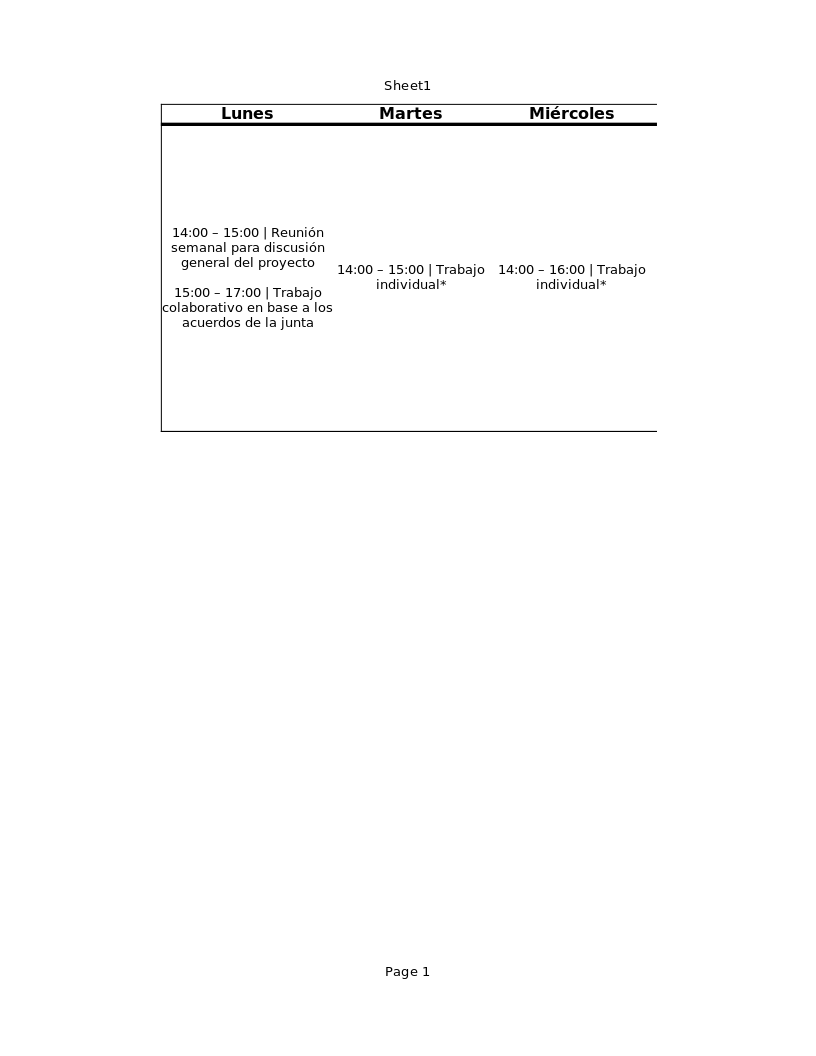
\includegraphics[scale=0.6]{img/horario.png}
 % horario.png: 1080x400 px, 72dpi, 38.10x14.11 cm, bb=0 0
 \caption{Horario semanal.}
 \label{fig: horario}
\end{figure}

\begin{table}[hb!]
\centering 
\begin{tabular}{c|l} 
\label{table: calendar} 
Fecha & Avances de proyecto\\ 
\hline 
25-sep & An\'alisis y ecuaciones del sistema\\
04-oct & Primer prototipo de animaci\'on\\
10-oct & Simulador terminado, controladores en etapa de 
prueba\\
13-oct & Manual, reporte y presentaci\'on listos para 
entrega de medio t\'ermino\\
18-oct & Correcciones al simulador, verificaci\'on del 
simulador\\
22-oct & Obtenci\'on de gr\'aficas para lazo abierto y 
lazo cerrado\\
10-nov & Visualizador y animacio\'on terminada\\
15-nov & Interfaz gr\'afica terminada\\
25-nov & Manual, reporte y presentaci\'on listos para 
entrega final\\

\hline 
\end{tabular} 
\caption{Fechas l\'imite.} 
\end{table}
